\subsection{Вариант}
Вариант №9. Подсистема управления доступом для системы рекрутинговой организации, которая 
обрабатывает ПДн работников и специальные данные 100001 клиентов. 

Определим следующие пункты для составления итогового списка требований:
\begin{itemize}
  \item[1.] класс АC, базовые требования;
  \item[2.] свойства информации;
  \item[3.] класс защищенности СВТ;
  \item[4.] ГИС или ИСПДн; 
  \item[5.] уровень защищенности ИС.
\end{itemize}

%  Определение 
%  -- класс АC, базовые требования (1Г)
%  -- Класс защищенности СВТ (5)
%  -- Определить ГИС или ИСПДн и наверное требования к нему
%  -- Уровень защищенности ИС (2)
 

\subsection{Теоретическая часть}
\subsubsection{Класс АС и базовые требования к подсистеме}
Согласно документу <<Автоматизированные системы. Защита от несанкционированного
доступа к информации. Классификация автоматизированных систем
и требования по защите информации>>, пункт 1.9, система  имеет класс \textbf{1Г} т.к она 
обрабатывает персональные данные и специальные, также является многопользовательской системой с разными полномочиями [7].

В пункт 2.10 документа выделяются следующее базовые требование к подсистемам для данного класса (Рис. 9).

\begin{figure}[H]
  \centering
  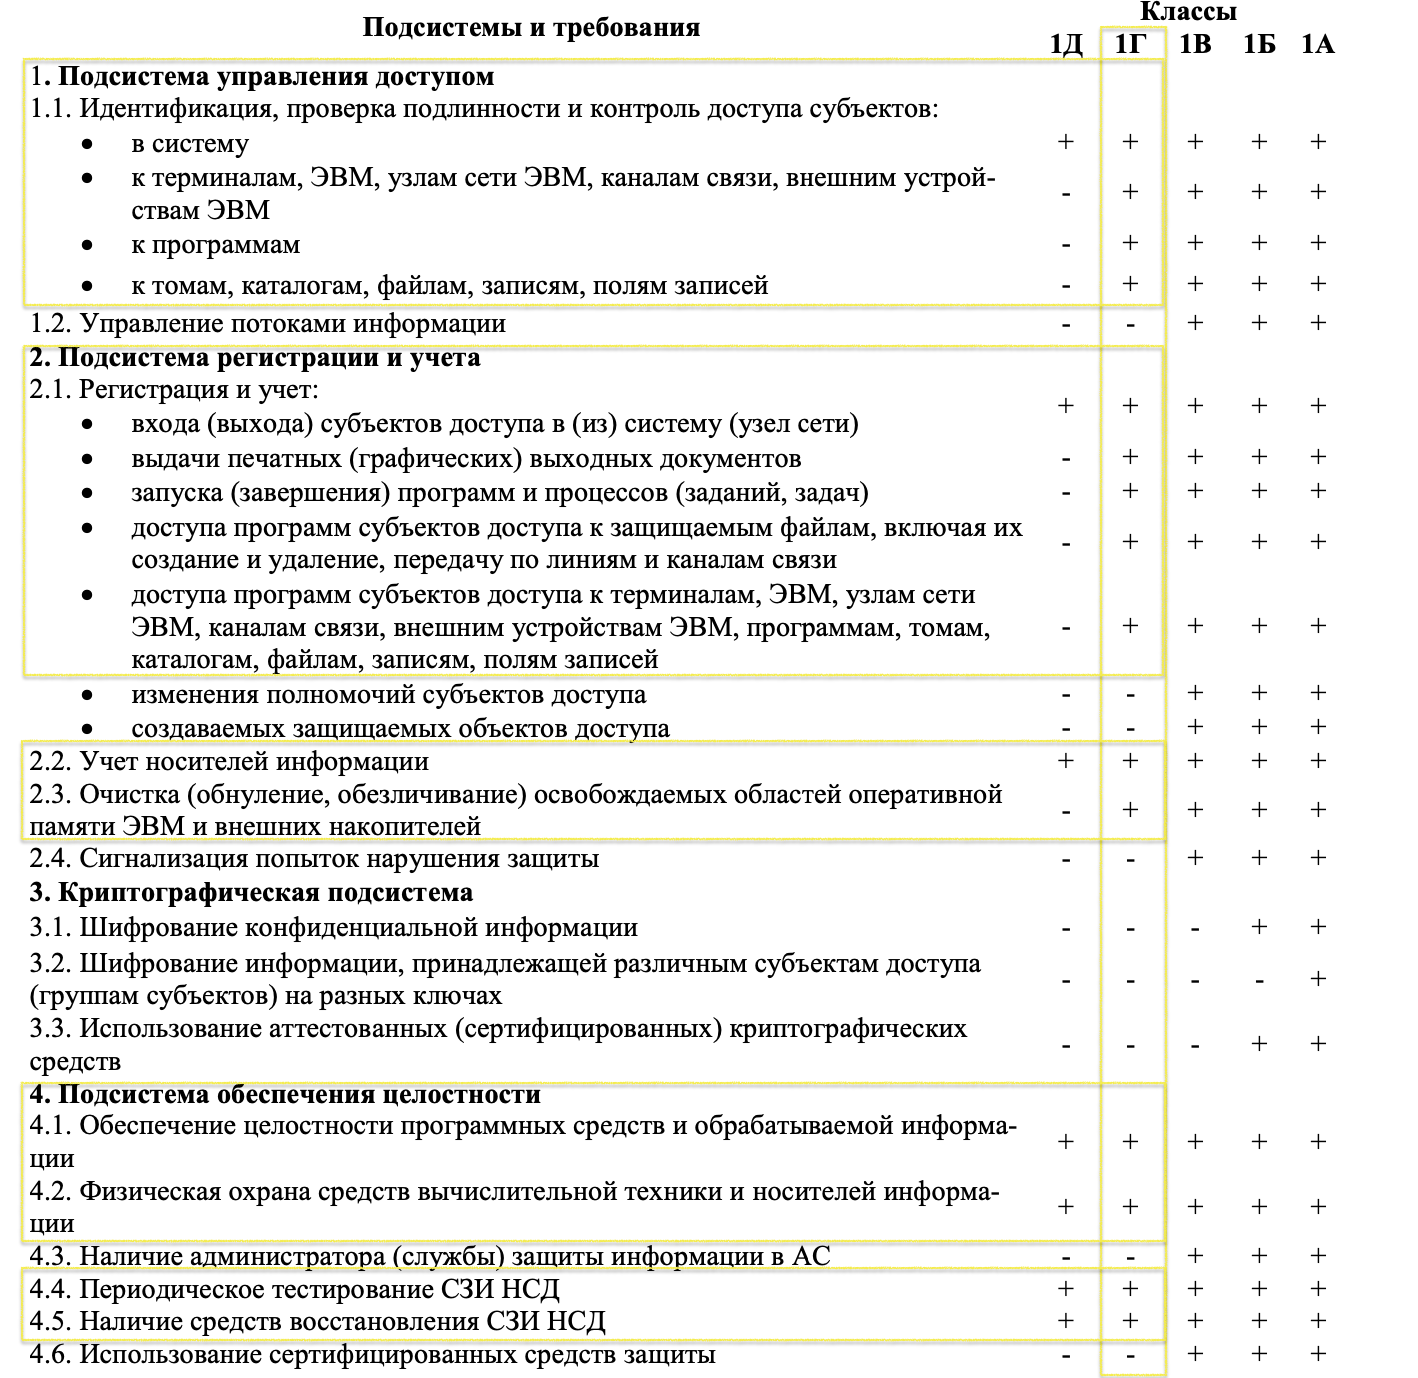
\includegraphics[width=1.1\textwidth]{pict/20}
  \caption{Требования к подсистемам}
  \label{fig:1}
\end{figure}

\textbf{Подсистема управления доступом:}
\begin{itemize}
  \item[--] должна осуществляться идентификация и проверка подлинности субъектов доступа при входе в систему по идентификатору 
  (коду) и паролю условно-постоянного действия, длиной не менее шести буквенно-цифровых символов;
  \item[--] должна осуществляться идентификация терминалов, ЭВМ, узлов сети ЭВМ, каналов связи, внешних устройств ЭВМ по логическим именам;
  \item[--] должна осуществляться идентификация программ, томов, каталогов, файлов, записей, полей записей по именам;
  \item[--] должен осуществляться контроль доступа субъектов к защищаемым ресурсам в соответствии с матрицей доступа.
\end{itemize}
\textbf{Подсистема регистрации и учета:}

Должна осуществляться регистрация входа (выхода) субъектов доступа в
систему (из системы), либо регистрация загрузки и инициализации
операционной системы и ее программного останова. Регистрация выхода из
системы или останова не проводится в моменты аппаратурного отключения
АС. В параметрах регистрации указываются:
\begin{itemize}
  \item[--] дата и время входа (выхода) субъекта доступа в систему (из системы) или
  загрузки (останова) системы;
  \item[--] результат попытки входа: успешная или неуспешная;
  \item[--] идентификатор (код или фамилия) субъекта, предъявленный при попытке
  доступа;
  \item[--] код или пароль, предъявленный при неуспешной попытке;
  \item[--] должна осуществляться регистрация выдачи печатных (графических) 
  документов на "твердую" копию. В параметрах регистрации указываются:
  дата и время выдачи (обращения к подсистеме вывода);
  спецификация устройства выдачи [логическое имя (номер) внешнего устройства]; 
  краткое содержание (наименование, вид, шифр, код) и уровень конфиденциальности
  документа;
  идентификатор субъекта доступа, запросившего документ;
  \item[--] должна осуществляться регистрация запуска (завершения) программ и процессов
  (заданий, задач), предназначенных для обработки защищаемых файлов. В параметрах 
  регистрации указываются: дата и время запуска, имя (идентификатор) программы (процесса, задания),
  идентификатор субъекта доступа, запросившего программу (процесс, задание), результат запуска (успешный, неуспешный - несанкционированный);
  \item[--] должна осуществляться регистрация попыток доступа средств 
  к защищаемым файлам. В параметрах регистрации указываются: дата и время попытки 
  доступа к защищаемому файлу с указанием ее результата: успешная, неуспешная,
  идентификатор субъекта доступа, спецификация защищаемого файла;
  \item[--] должна осуществляться регистрация попыток доступа средств к следующим 
  дополнительным защищаемым объектам доступа: терминалам, ЭВМ, узлам сети ЭВМ, линиям (каналам) связи, 
  внешним устройствам ЭВМ, программам, томам, каталогам, файлам, записям, полям записей. В параметрах регистрации указываются:
  дата и время попытки доступа к защищаемому объекту с указанием ее результата: успешная, неуспешная;
  идентификатор субъекта доступа;
  спецификация защищаемого объекта [логическое имя (номер)];
  \item[--] должен проводиться учет всех защищаемых носителей информации с помощью их
  маркировки и с занесением учетных данных в журнал (учетную карточку);
  \item[--] учет защищаемых носителей должен проводиться в журнале (картотеке) с регистрацией
   их выдачи (приема);
  \item[--] должна осуществляться очистка (обнуление, обезличивание) освобождаемых 
  областей оперативной памяти ЭВМ и внешних накопителей. Очистка осуществляется однократной 
  произвольной записью в освобождаемую область памяти, ранее использованную для хранения 
  защищаемых данных (файлов);
\end{itemize}

\textbf{Подсистема обеспечения целостности:}

Должна быть обеспечена целостность программных средств СЗИ НСД,
обрабатываемой информации, а также неизменность программной среды. При этом:

\begin{itemize}
  \item[--] целостность СЗИ НСД проверяется при загрузке системы по контрольным
  суммам компонент СЗИ;
  \item[--] целостность программной среды обеспечивается использованием
  трансляторов с языков высокого уровня и отсутствием средств модификации
  объектного кода программ в процессе обработки и (или) хранения
  защищаемой информации;
  \item[--] должна осуществляться физическая охрана СВТ (устройств и носителей
  информации), предусматривающая контроль доступа в помещения АС
  посторонних лиц, наличие надежных препятствий для несанкционированного
  проникновения в помещения АС и хранилище носителей информации,
  особенно в нерабочее время;
  \item[--] должно проводиться периодическое тестирование функций СЗИ НСД при
  изменении программной среды и персонала АС с помощью тест-программ,
  имитирующих попытки НСД;
  \item[--] должны быть в наличии средства восстановления СЗИ НСД,
  предусматривающие ведение двух копий программных средств СЗИ НСД и
  их периодическое обновление и контроль работоспособности.
\end{itemize}

\subsubsection{Свойства информции}

Так как система обрабатывает специальные персональные данные пользователей, а также 
данные своих сотрудников, что по Указе Президента РФ от 6 марта 1997 г. № 188 
"Об утверждении перечня сведений конфиденциального характера", персональные данные являются конфиденциальной информацией 
и должны защищаться, поэтому вместе с целостностью и доступностью необходимо обеспечить конфиденциальность [8].

\subsubsection{Класс защищенности СВТ}

Согласно документу <<РУКОВОДЯЩИЙ ДОКУМЕНТ. Средства вычислительной техники.
Защита от несанкционированного доступа к информации. Показатели
защищенности от несанкционированного доступа к информации>>, пункт 2.1.1 можно 
определить \textbf{5} класс защищенности СВТ [9].
Поскольку в отличие от 6 класса, 5 требует наличия контроля целостности средств 
СЗИ, что соответствует требованиям 
из 1.2.1, но в отличие от 4 класса, 5 не требует защиту работы с физическим носителем,
 сопоставления пользователя с устройством и изоляцию модулей (Рис. 10).

\begin{figure}[H]
  \centering
  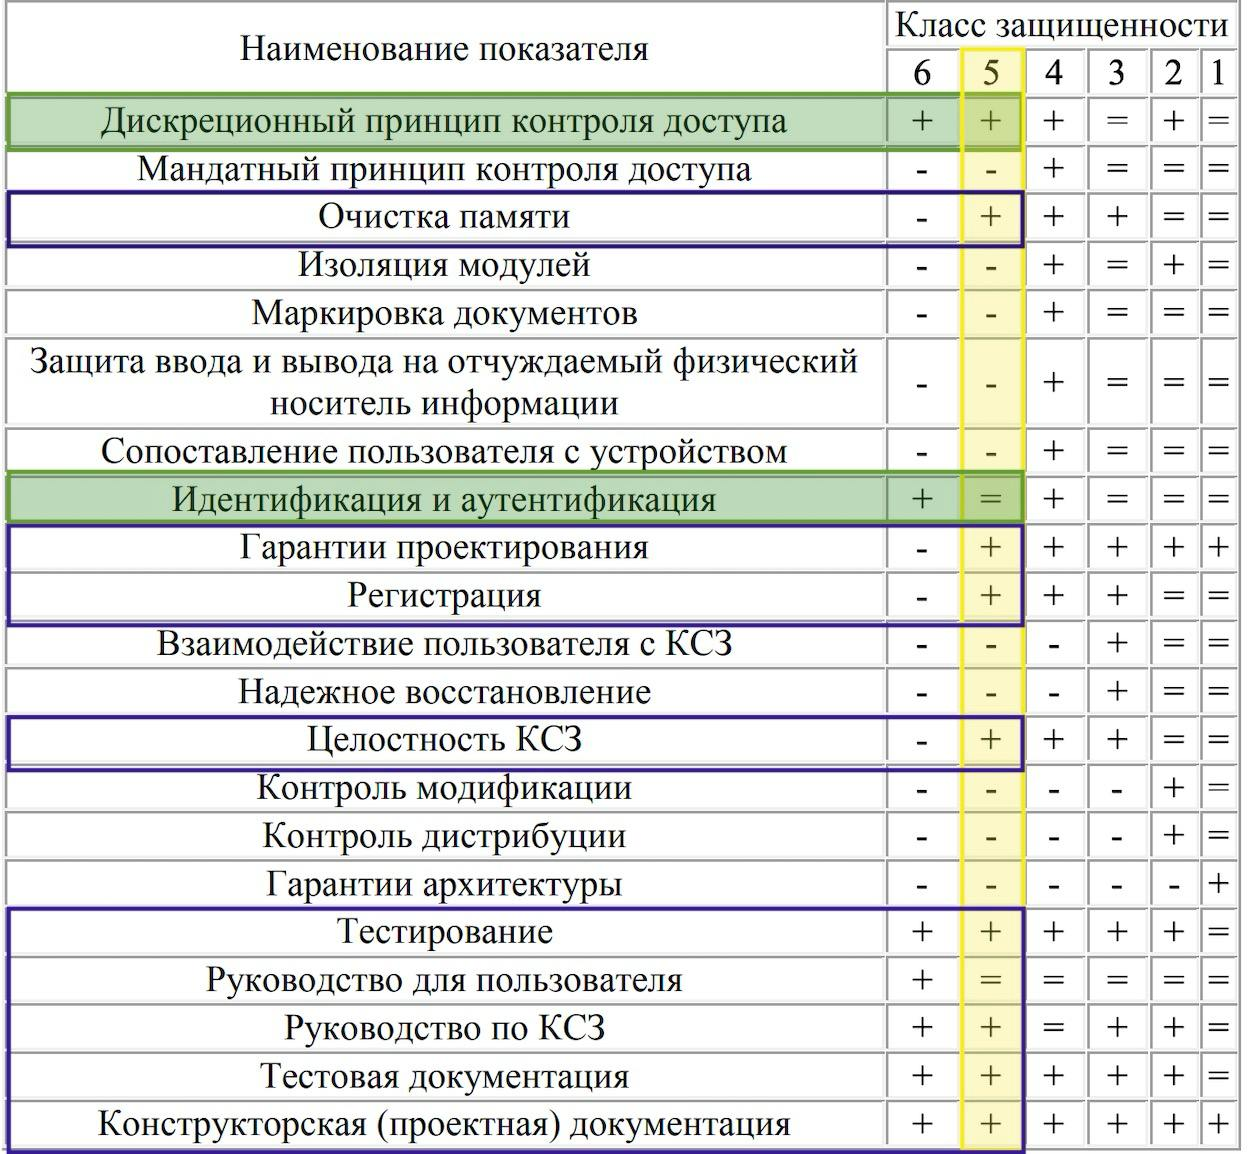
\includegraphics[width=0.7\textwidth]{pict/3}
  \caption{Синий -- требования к системе, зеленый -- к подсистеме управления доступом и идентификации}
  \label{fig:3}
\end{figure}

\textbf{Дискреционный принцип контроля доступа}

КСЗ должен контролировать доступ наименованных субъектов
(пользователей) к наименованным объектам (файлам, программам, томам и
т.д.). Для каждой пары (субъект – объект) в СВТ должно быть задано явное и
недвусмысленное перечисление допустимых типов доступа (читать, писать и
т.д.), т.е. тех типов доступа, которые являются санкционированными для
данного субъекта (индивида или группы индивидов) к данному ресурсу СВТ
(объекту).

КСЗ должен содержать механизм, претворяющий в жизнь дискреционные
правила разграничения доступа.

Контроль доступа должен быть применим к каждому объекту и каждому
субъекту (индивиду или группе равноправных индивидов).

Механизм, реализующий дискреционный принцип контроля доступа,
должен предусматривать возможности санкционированного изменения ПРД,
в том числе возможность санкционированного изменения списка
пользователей СВТ и списка защищаемых объектов.

Права изменять ПРД должны предоставляться выделенным субъектам
(администрации, службе безопасности и т.д.).

Дополнительно должны быть предусмотрены средства управления,
ограничивающие распространение прав на доступ.

\textbf{Очистка памяти}

При первоначальном назначении или при перераспределении внешней
памяти КСЗ должен предотвращать доступ субъекту к остаточной
информации.

\textbf{Идентификация и аутентификация}

КСЗ должен требовать от пользователей идентифицировать себя при
запросах на доступ. КСЗ должен подвергать проверке подлинность
идентификации – осуществлять аутентификацию. КСЗ должен располагать
необходимыми данными для идентификации и аутентификации. КСЗ должен
препятствовать доступу к защищаемым ресурсам неидентифицированных
пользователей и пользователей, подлинность идентификации которых при
аутентификации не подтвердилась.

\textbf{Гарантии проектирования}

На начальном этапе проектирования СВТ должна быть построена модель
защиты. Модель должна включать в себя ПРД к объектам и
непротиворечивые правила изменения ПРД.

\textbf{Регистрация}

КСЗ должен быть в состоянии осуществлять регистрацию следующих
событий:
\begin{itemize}
  \item [--] использование идентификационного и аутентификационного механизма;
  \item [--] запрос на доступ к защищаемому ресурсу (открытие файла, запуск
  программы и т.д.);
  \item [--] создание и уничтожение объекта;
  \item [--] действия по изменению ПРД.
\end{itemize}

Для каждого из этих событий должна регистрироваться следующая
информация:
\begin{itemize}
  \item [--] дата и время;
  \item [--] субъект, осуществляющий регистрируемое действие;
  \item [--] тип события (если регистрируется запрос на доступ, то следует отмечать
   объект и тип доступа);
  \item [--] успешно ли осуществилось событие (обслужен запрос на доступ или нет).
\end{itemize}
КСЗ должен содержать средства выборочного ознакомления с
регистрационной информацией.

\textbf{Целостность КСЗ}

В СВТ пятого класса защищенности должны быть предусмотрены
средства периодического контроля за целостностью программной и
информационной части КСЗ.

\textbf{Тестирование}

В СВТ пятого класса защищенности должны тестироваться:
\begin{itemize}
  \item [--] реализация ПРД (перехват явных и скрытых запросов на доступ,
  правильное распознавание санкционированных и несанкционированных
  запросов, средства защиты механизма разграничения доступа,
  санкционированные изменения ПРД);
  \item [--] успешное осуществление идентификации и аутентификации, а также их
  средства защиты;
  \item [--] очистка памяти в соответствии с п. 2.3.2;
  \item [--] регистрация событий в соответствии с п. 2.3.5, средства защиты
  регистрационной информации и возможность санкционированного 
  ознакомления с ней;
  \item [--] работа механизма, осуществляющего контроль за целостностью КСЗ.
\end{itemize}

\textbf{Руководство пользователя}

Документация на СВТ должна включать в себя краткое руководство для
пользователя с описанием способов использования КСЗ и его интерфейса с
пользователем..

\textbf{Руководство по КСЗ}

Данный документ адресован администратору защиты и должен
содержать:

\begin{itemize}
  \item [--] описание контролируемых функций;
  \item [--] руководство по генерации КСЗ;
  \item [--] описания старта СВТ, процедур проверки правильности старта, процедур
  работы со средствами регистрации.
\end{itemize}


\textbf{Тестовая документация}

Должно быть предоставлено описание тестов и испытаний, которым
подвергалось СВТ (в соответствии с требованиями п.2.3.7), и результатов
тестирования.

\textbf{Конструкторская и проектная документация}

Должна содержать:
\begin{itemize}
  \item [--] описание принципов работы СВТ;
  \item [--] общую схему КСЗ;
  \item [--] описание интерфейсов КСЗ с пользователем и интерфейсов модулей КСЗ;
  \item [--] модель защиты;
  \item [--] описание механизмов контроля целостности КСЗ, очистки памяти,
  идентификации и аутентификации.
\end{itemize}


\subsubsection{ГИС или ИСПДн}

Так как моя организация "---рекрутинговое агентство, система которого обрабатывает специальные ПДн и сотрудников,
что не является государственной информацией, то система является ИСПДн.


\subsubsection{Уровень защищенности ИС}
Согласно постановлению от 1 ноября 2012 г. N 1119 <<ОБ УТВЕРЖДЕНИИ ТРЕБОВАНИЙ
К ЗАЩИТЕ ПЕРСОНАЛЬНЫХ ДАННЫХ ПРИ ИХ ОБРАБОТКЕ В ИНФОРМАЦИОННЫХ СИСТЕМАХ ПЕРСОНАЛЬНЫХ ДАННЫХ>>,
пункт 10, уровень защищенности можно определить как \textbf{УЗ 2} [10]. Так как система
подходит под одно из условий этого уровня, системе не грозят угрозы 1 и 2 класса, т.к используется лицензированное
ПО и ОС (Рис. 11).

\begin{figure}[H]
  \centering
  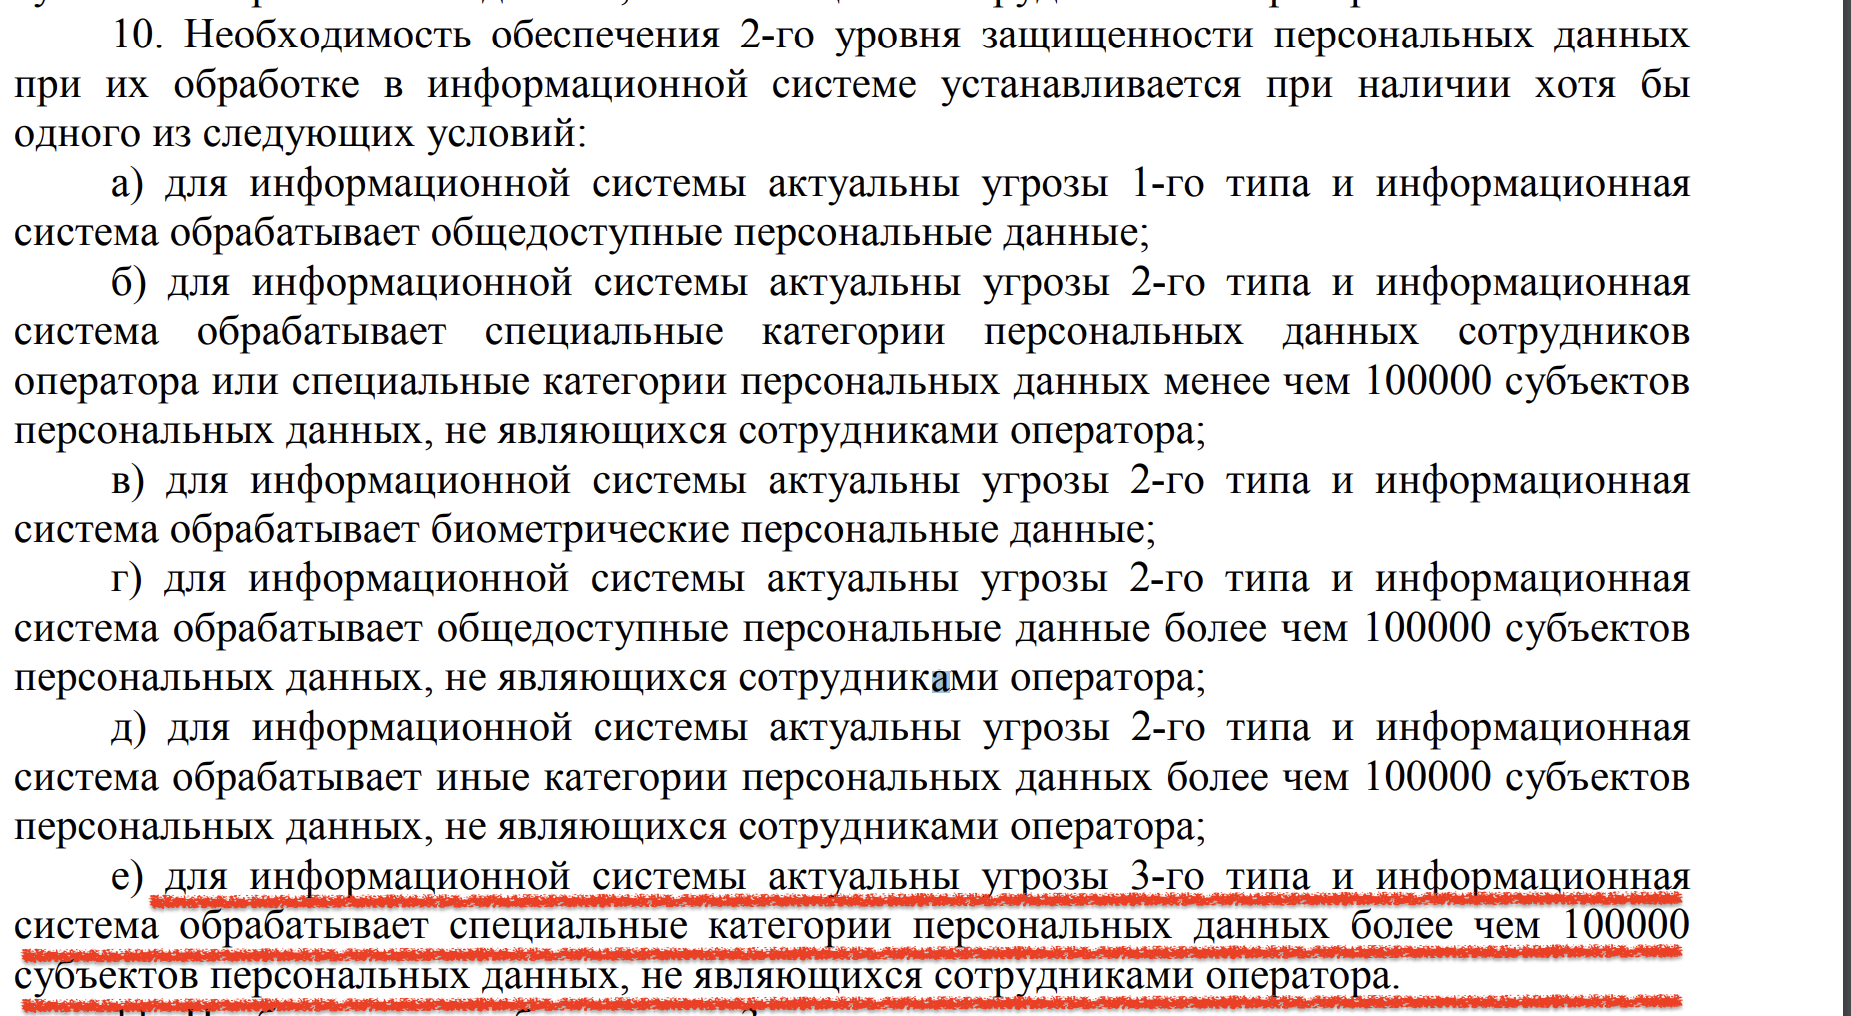
\includegraphics[width=1.1\textwidth]{pict/6}
  \caption{Условия для УЗ 2}
  \label{fig:4}
\end{figure}

Требования, которы выставляются для данного уровня защищенности, пункты 13-15 (Рис. 12). 

\begin{figure}[H]
  \centering
  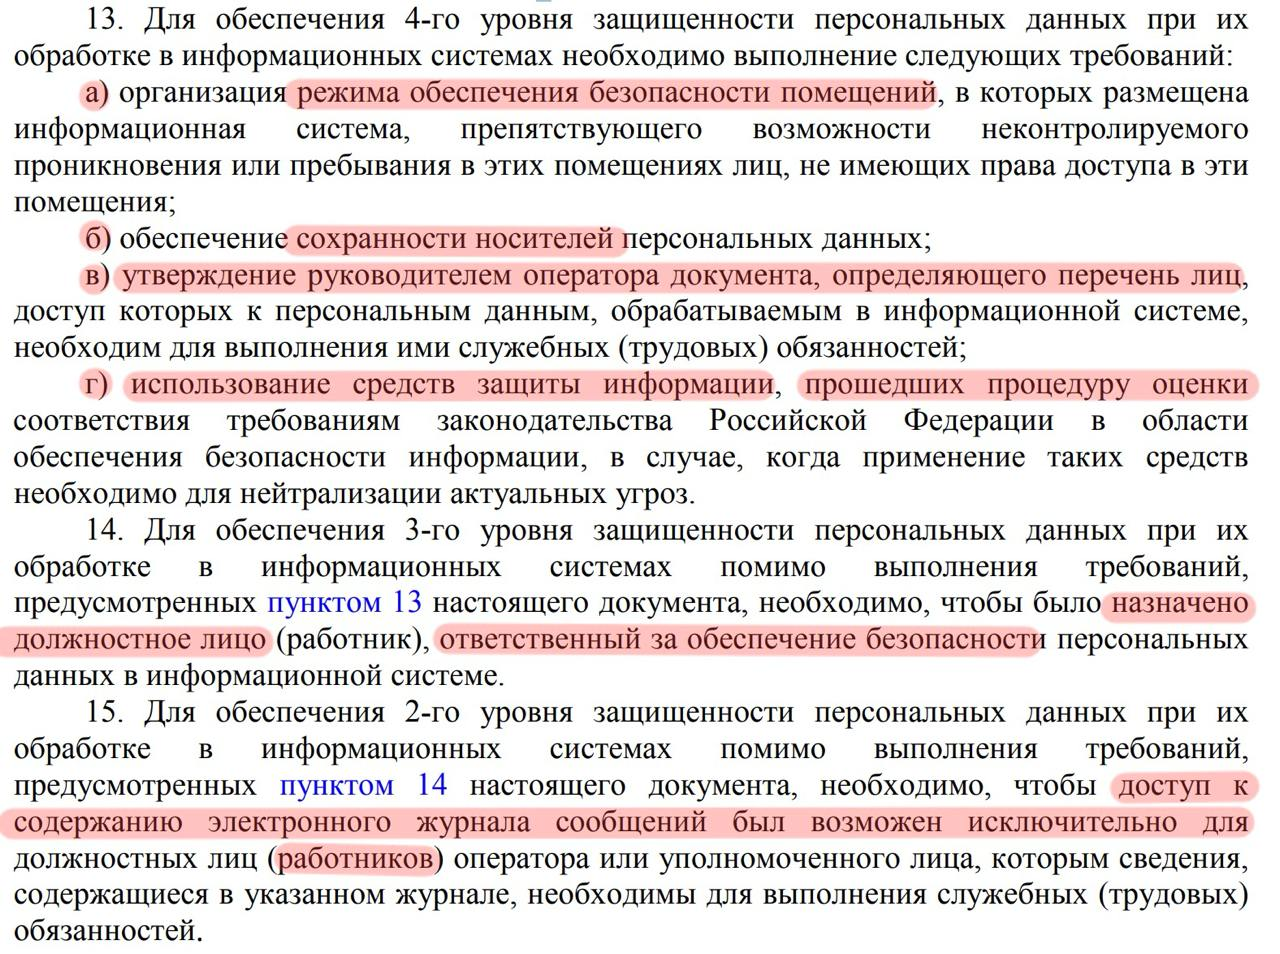
\includegraphics[width=1\textwidth]{pict/5}
  \caption{Требования для УЗ 2}
  \label{fig:5}
\end{figure}

\subsubsection{Требования для подсистемы управления доступом}
По итогу собранных требований, можно выделить список требований конкретно для
подсистемы управления доступом и данного задания:

\begin{itemize}
  \item[1.] Вход в систему по идентификатору (коду) и паролю условно"=постоянного действия, длиной не менее шести буквенно"=цифровых символов;
  \item[2.] Контроль доступа субъектов к защищаемым ресурсам в соответствии с матрицей доступа;
  \item[3.] КСЗ должен содержать механизм, претворяющий в жизнь дискреционные
  правила разграничения доступа;
  \item[4.] Ограничение прав для пользователей, могут пенять права доступа только админы;
  \item[5.] Настройка доступа к электронному журналу сообщений только для субъектов, использующих их в работе;
  \item[6.] Доступ в систему только для аутентифицированных пользователей; 
  \item[7.] Ограничение неуспешных попыток входа в систему (доступа к информационной системе). 
\end{itemize}\newpage



% Вручную оформление ссылок не допускается

% \begin{figure}[H]
%   \centering
%   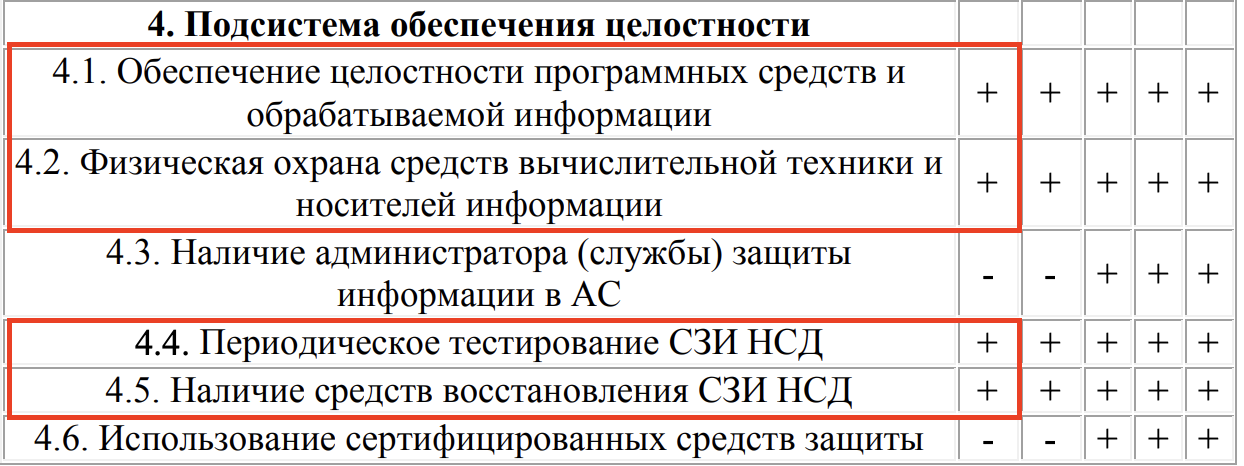
\includegraphics[width=1\textwidth]{pict/2}
%   \caption{принцип взаимодействия уровней приложения}
% \end{figure}


